\chapter{多元函数微分学}

\section{基本概念}

\subsection{导数与微分}

\begin{definition}{方向导数, 偏导数}
    设开集$E \subseteq \R ^n$, 函数$f:E \to \R$, $x_0 \in E , v \in \R ^n$. 定义$f$在$x_0$处\textit{沿$v$的方向导数}为下列极限(如果存在): $$\frac{\p f}{\p v}(x_0) := \lim_{h \to 0} \frac{f(x_0+hv)-f(x_0)}{h}.$$
    特别地, 令$x_i$为第$i$个坐标为$1$, 其余为$0$的单位向量, 则称沿$x_i$的方向导数为该方向上的\textit{偏导数}. 
\end{definition}
\begin{remark}
	亦可用$\frac{\p}{\p x_i}$表示$x_i$, 以此区别$\{ x_i \}$是$f$定义域的一组基或是$\dif f$定义域的一组基, 详见后文. 
\end{remark}

偏导数是容易求得的: 由于$h$不影响$x_i$方向以外的方向, 只需将整个函数视作关于$x_i$的一元函数求导即可. 

稍后会验证(实际上是显然的), 当$f$可微时成立$\frac{\p f}{\p v_1}(x_0) + \frac{\p f}{\p v_2}(x_0) = \frac{\p f}{\p (v_1+v_2)}(x_0)$. 此时只需计算$f$的所有偏导数即可得到任意方向导数. 反过来, 当$f$不可微时, 即使偏导数均存在, 也不能保证方向导数存在(更不用说如此计算了). 

\begin{example}
	考虑$f(x,y)=\begin{cases}
		\frac{xy}{x^2+y^2} & (x,y) \neq (0,0) \\ 0 & (x,y)=(0,0)
	\end{cases}$. 则$f$的两个偏导数在$(0,0)$均为$0$, 但是$\frac{\p f}{\p v} = \lim_{h \to 0} \frac{v^1v^2}{h((v^1)^2+(v^2)^2)}$不存在, 其中$v_1v_2 \neq 0$. 
\end{example}

方向导数有清晰的几何意义: 设曲线$\gamma :(-\delta,\delta) \to \R ^n$是$C^1$的. 我们有$$\frac{\dif}{\dif t} \big|_{t=0} (f|_{\rge \gamma} \circ \gamma) = \frac{\p f}{\p \gamma '(0)} (\gamma (0)). $$
这一式子不难验证. 在图像上(这里我们以$\R ^2$模拟$\R ^n$, 并将$\R$置于$\R ^n$的法向量方向上), 这一式子大概在说: 在$\gamma '(0)$方向上求导, 相当于考虑$f$在$\gamma$这一条曲线之上的部分(实际上是$\R \to \R$的, 但在图像上看起来像是曲线), 再在这部分上求$0$处的导数. 换句话说, 针对一个方向$v$, 我们只需考虑顺着该方向上$f$的行为即可. 

\begin{figure}[H]
	\centering
	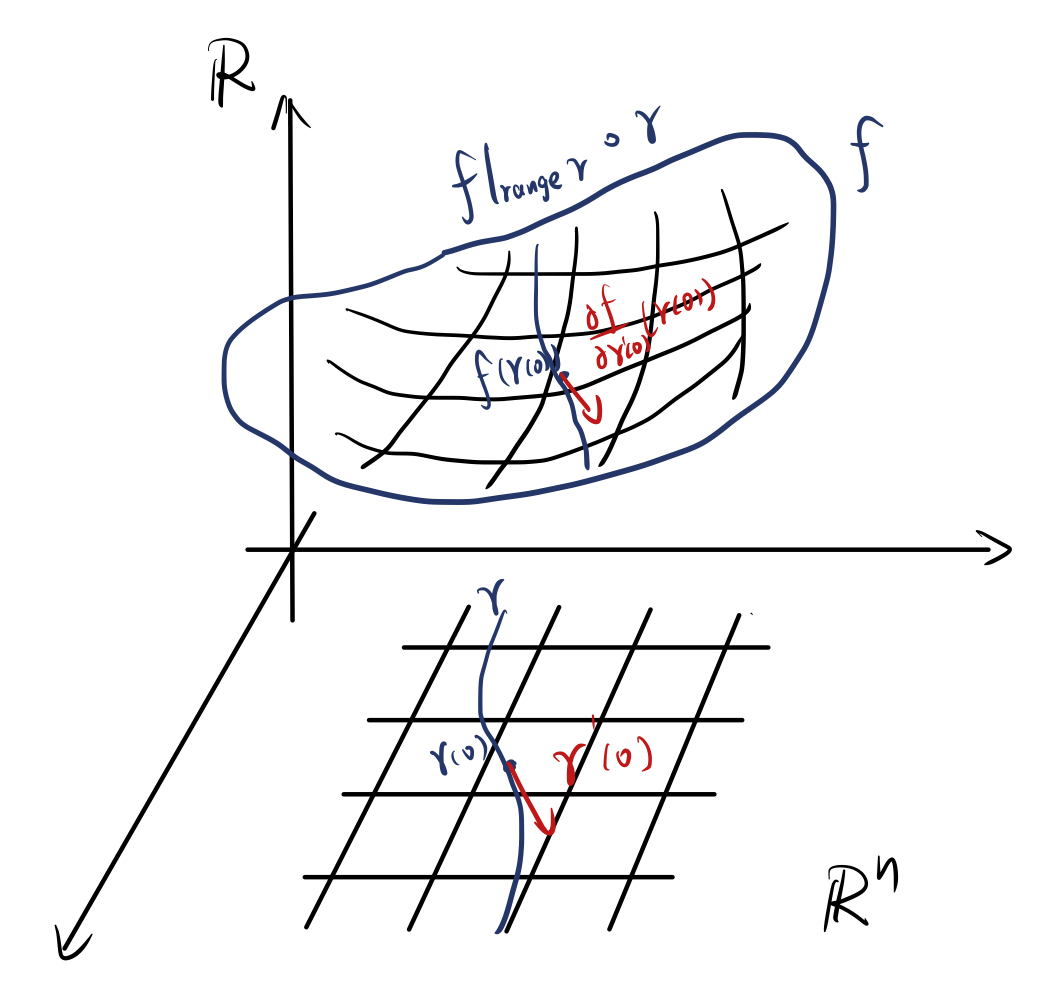
\includegraphics[width=7cm]{attachment/IMG_3923.jpg}
	\caption{方向导数的几何意义}
\end{figure}

这里需要就多元函数的图像一事做些补充. 

首先, 若是从函数角度来看, 此处的$\R ^n \times \R$就是$(x_0,f(x_0))$所生活的空间\footnote{这部分内容不会严格区分$\R ^n \times \R ^m$与$\R ^{n+m}$. }, $f$在这里形成了图像$\Gamma _f$. 容易感知到, 两个字空间$\R$与$\R ^n$“天生”地不相干, 或者说这种描述严重依赖于坐标系的选取. 然而, 正如我们乐于将$\R \times \R = \R ^2$视作一个正常的平面, 这里的$\R ^n \times \R$也可视作一整个空间, 即任意一个$\R$上的$n+1$维向量空间, 这就不依赖坐标系了. 如果的确需要在这一空间中描述某个形状, 此时应当使用(某个坐标系下的)隐函数$f(x_0^1,\cdots ,x_0^n,x_0^{n+1})=0$. 也就是在这两种描述中互相转化: 
\begin{center}
	$\displaystyle \{ (x,f(x)) \in \R ^n \times \R : x \in \R \} = \{ (x,y) \in \R ^n \times \R : F(x,y)=0,F(x,y)=(0,y-f(x)) \}.$
\end{center}
作为例子, $\R ^3$中的单位球面$S^2$可表示为$2$个函数图像$f_+(\R ^2),f_-(\R ^2)$的并(其中$f_{\pm} (x,y)= \pm \sqrt{1-x^2-y^2}$), 亦可表示为$f^{-1}(\{ 0 \})$(其中$f(x,y,z) = x^2+y^2+z^2-1$). 大多数时候后者的形式更加简洁且易于推广; 并且我们很快就会看到, 利用$f^{-1}(S)$的形式更容易判断该形状是否是光滑子流形, 并且求出其维数. 

其次, 在一元微分学部分, 我们体会到了“导数”就等于“切线斜率”的想法. 我们希望在多元微分学中找到对应的想法. 

将斜率放在我们强行捏造的图像上, 它表示$x$轴(定义域)上的单位距离对应$y$轴(值域)距离的值, 即两点$(x_1,f(x_1)),(x_2,f(x_2))$的斜率为$\frac{f(x_2)-f(x_1)}{x_2-x_1}$, 这里最关键的一步在于单位化. 若要将其推广至多元函数, 由于单位化的操作无法对两个向量实施, 我们不得不单独考虑一个方向上的比值, 再将这些比值按方向加总(形象地说就是将$x$轴绕$\R ^n$转一圈再将结果矢量求和). 问题在于, 加总后的结果还能反映每个方向的情况吗? 

幸好我们研究的是向量空间$\R ^n$. 线性代数告诉我们的确可以(一组基和全体向量等价). 此时不难猜测点$(x_1,f(x_1)),(x_2,f(x_2))$间的“斜率”是一个$\R ^n$的向量$k$, 且$k= \frac{f(x_2^1)-f(x_1^1)}{x_2^1-x_1^1} \frac{\p}{\p x_1} + \cdots + \frac{f(x_2^n)-f(x_1^n)}{x_2^n-x_1^n}\frac{\p}{\p x_n}$. 更进一步, 当$f$存在所有偏导数时, 在某点$x_0$处的斜率就是$\frac{\p f}{\p x_1}(x_0) \frac{\p}{\p x_1} + \cdots + \frac{\p f}{\p x_n}(x_0) \frac{\p}{\p x_n}$. 进而, 可以定义$f$的\textit{梯度}$\nabla f$使得$\nabla f(x_0)$是$x_0$处的斜率的转置\footnote{即$\nabla f(x_0)$是一个行向量. }. 

需要注意, 这里我们用一个$\R ^n$上特定的坐标系描述$f$. 实际上更换坐标系并不会影响梯度, 这从几何图像上是显然的. 另外, 在引入切空间的概念后, 可以证明一个优美的结论: $(\nabla f(x_0))^{\T}$就是切空间$T_{x_0}(f^{-1}(0))$的法向量. 

回到正题, 我们来定义多元函数的微分. 

\begin{definition}{微分}
	设开集$E \subseteq \R ^n$, 函数$f: E \to \R$, $x_0 \in E$, $v \in \R ^n$. 称$f$在$x_0$处\textit{可微}, 若存在线性映射$T$使得$$f(x_0+v) = f(x_0) + T(v) + o(v),\qquad v \to 0$$
	对任意的$v$成立. 此时记$f$的\textit{微分}$\dif f$满足$\dif f(x_0)=T$. 
\end{definition}
\begin{remark}
	一个等价定义是: 对于任意单位向量$v$与任意实数$h>0$, 成立$f(x_0+hv) = f(x_0) + \dif f(x_0) (hv) + o(hv),h \to 0$. 这种定义可将微分拆分到不同方向考虑. 
\end{remark}
\begin{remark}
	微分的定义并不依赖坐标系(任意赋范向量空间之间均可定义). 这也是多元函数的微分与导数始终存在很大差距的根本原因. 
\end{remark}

如上所述, 将微分的定义式写成$n$个方程, 实际上我们可以得到: 若$f$在$x_0$可微, 则$$ \frac{\p f}{\p v}(x_0) = \dif f(x_0)(v) = \sum_{i=1}^{n} \frac{\p f}{\p x_i}(x_0)v^i.$$
特别地, 此时$f$的所有方向导数均存在. 这也证明了上面提到过的式子$\frac{\p f}{\p v_1}(x_0) + \frac{\p f}{\p v_2}(x_0) = \frac{\p f}{\p (v_1+v_2)}(x_0)$. 

反过来, 我们好奇偏导数的存在性将如何影响可微性. 

\begin{proposition}{}
	设开集$E \subseteq \R ^n$, 函数$f: E \to \R$, $x_0 \in E$. 若$f$在$x_0$处的所有偏导数在$x_0$附近均存在且$\frac{\p f}{\p x_i}$均连续, 则$f$在$x_0$处可微. 
\end{proposition}
\begin{remark}
	请注意, 该命题的条件是偏导数在$x_0${\color{blue} 附近}存在. 直观上来看, 一个点处的偏导数并不能给出什么有用的信息, 但是一片区域上的偏导数能够描述函数的某种趋势. 
\end{remark}
\begin{remark}
	一个弱化的命题是: 当所有偏导数存在且有界时, $f$在$x_0$处连续. 证明方法类似. 
\end{remark}
\begin{proof}
	我们尝试证明$r(v)=f(x_0+v)-f(x_0)-\sum_{i=1}^{n} \frac{\p f}{\p x_i}(x_0)v^i$在$v \to 0$时是$o(v)$的. 计算可得: 
	\begin{align*}
		r(v) &= f(x_0^1+v^1,\cdots ,x_0^n+v^n) - f(x_0^1,\cdots ,x_0^n) - \sum_{i=1}^{n} \frac{\p f}{\p x_i}(x_0)v^i \\
		&= \sum_{i=1}^{n} \left( f(\cdots ,x_0^{i-1}+v^{i-1},{\color{blue} x_0^{i}+v^{i} },x_0^{i+1},\cdots) - f(\cdots ,x_0^{i-1}+v^{i-1},{\color{blue}x_0^{i} },x_0^{i+1},\cdots) - \frac{\p f}{\p x_i}(x_0)v^i \right) \\
		&= \sum_{i=1}^{n} \left( \frac{\p f}{\p x_i}(\xi _i)v^i - \frac{\p f}{\p x_i}(x_0)v^i \right). 
	\end{align*}
	其中, 最后一步对蓝色部分使用一元函数的Lagrange中值定理. 由Cauchy不等式可得$|r(v)| \leq |v| \cdot \sum_{i=1}^{n}\left| \frac{\p f}{\p x_i}(\xi _i) - \frac{\p f}{\p x_i}(x_0) \right|$, 这就证明了原命题. 
\end{proof}

最后, 结合先前(第5章)提到的想法: 向量值函数的极限是按分量计算的, 不难得到(多元向量值函数的)微分在某一坐标系下的具体表达. 

\begin{proposition}{Jacobi矩阵}
	设$f:\R ^m \supseteq E \to \R ^n$, 则$f$在$x_0 \in E$处可微等价于$f$的每个分量$f_i$在$x_0$可微, 且此时$\dif f (x_0)$可用$n \times m$的矩阵$$\left( \frac{\p f_i}{\p x_j}(x_0) \right)_{i=1,\cdots ,n \atop j=1,\cdots ,m}$$
	表示. 称该矩阵为$f$在$x_0$处的\textit{Jacobi矩阵}, 可记作$\mathrm{Jac} (f)(x_0)$. 
\end{proposition}

形式上, 不难得到: $$\mathrm{Jac}(f)(x_0) = \begin{pmatrix}
	\dfrac{\p f}{\p x_1} & \cdots & \dfrac{\p f}{\p x_m}
\end{pmatrix} = \begin{pmatrix}
	\nabla f_1(x_0) \\ \vdots \\ \nabla f_n(x_0)
\end{pmatrix}.$$

我们合理猜测Jacobi矩阵具有与一元函数微分算子相似的性质: 

\begin{proposition}{Jacobi算子的算术性质}
	设可微函数$f,g:\R ^m \supseteq E \to \R ^n$, 则有
	\begin{center}
		1) $\mathrm{Jac}(Af+Bg)=A\mathrm{Jac}(f)+B\mathrm{Jac}(g)$;\qquad 2) $\mathrm{Jac}(f^{\T}g) = g^{\T}\mathrm{Jac}(f) + f^{\T}\mathrm{Jac}(g)$. 
	\end{center}
	特别地, 从形式上的结果可以看出$Af+Bg$与$f^{\T}g$可微. 
\end{proposition}
\begin{proof}
	以1)的齐次性部分为例. 记$A$是$s \times m$矩阵, 则$$\mathrm{Jac}(Af)(x_0)(i;j) = \mathrm{Jac}\begin{pmatrix}
		\sum_{k=1}^{m} A(1;k)f_k \\ \vdots \\ \sum_{k=1}^{m} A(s;k)f_k
	\end{pmatrix}(x_0)(i;j) = \frac{\p (\sum_{k=1}^{m} A(i;k)f_k)}{\p x_j}(x_0) {\color{blue}=} \sum_{k=1}^{m}A(i;k) \frac{\p f_k}{\p x_j}(x_0).$$
	不难发现等式右侧就是$A\mathrm{Jac}(f)(x_0)(i;j)$. 注意, 证明中实际上用到了偏导算子的线性(蓝色等号), 从这里也能看出来这一命题对有限维条件的依赖性. 
\end{proof}

特别地, 对于实值函数, 还有$\mathrm{Jac}(f/g) = \frac{1}{g^2} (g\mathrm{Jac}(f)-f\mathrm{Jac}(g))$成立. 

然而, 以某一坐标系为基础总是令人不爽的. 对于一般的定义在(无限维)赋范向量空间之间的映射, 我们仍应当仔细考察其可微性. 这里我们有两种方法解决问题. 

其一是试图将Jacobi矩阵推广到无限维赋范向量空间. 泛函分析会给出答案(简单来说, 这涉及到可微函数与线性映射的范数的定义). 

其二就是将投机取巧的Jacobi矩阵还原为线性映射$\dif f(x_0)$计算. 例如由$Af(x_0+v)-Af(x_0) = A\dif f(x_0) + o(Av)$可得$Af$可微且$\dif (Af) = A\dif f$. (若要考虑$f^{\T}g$的可微性, 需要先在该空间上定义合适的内积, 同样参考泛函分析)

\begin{proposition}{复合映射的微分}
	设$f:E _1 \to E _2,g:E _2 \to E _3$. 若$f$在$x_0$处可微, $g$在$f(x_0)$处可微, 则$g \circ f:E _1 \to E _3$在$x_0$处可微且满足
	\begin{center}
		$\displaystyle \dif (g \circ f) (x_0) = \dif g (f(x_0)) \circ \dif f(x_0).$
	\end{center}
\end{proposition}
\begin{remark}
	在有限维下, 即为$\displaystyle \mathrm{Jac}(g \circ f)(x_0)_{p \times m} = \mathrm{Jac}(g)(f(x_0))_{p \times n} \times \mathrm{Jac}(f)(x_0)_{n \times m}$. 
\end{remark}
\begin{proof}
	由可微性得$f(x_0+h) = f(x_0) + \dif f(x_0) h + o(h)$, $g(f(x_0)+h) = g(f(x_0)) + \dif g(f(x_0)) h + o(h)$. 则
	\begin{align*}
		g(f(x_0+h))-g(f(x_0)) &= g(f(x_0) + \dif f(x_0) h + o(h))-g(f(x_0)) \\
		&= \dif g(f(x_0)) (\dif f(x_0) h + o(h)) + o(\dif f(x_0) h + o(h)) \\
		&= \dif g (f(x_0)) \circ \dif f(x_0) h + o(h).
	\end{align*}
	这就证明了原命题. 
\end{proof}

\begin{corollary}{逆映射的微分}
	设$f:E _1 \to E _2$是可微的双射. 若$f^{-1}$也是可微的, 则对任意$x$有$\dif f(x)$可逆, 且$\dif (f^{-1})(y) = (\dif f (f^{-1}(y)))^{-1}$. 
\end{corollary}
\begin{remark}
	有限维时, 这蕴含了$x_0 \in E_1$处的切空间与$f(x_0)$处的切空间维数相等(根据后面的理论, 其实就是$E_1,E_2$维数相等); 无限维时, 若承认选择公理, 则这两个向量空间等价(线性同构). 
\end{remark}
\begin{proof}
	取$f,f^{-1}$, 利用上个命题, 有$\mathrm{Id} = \dif (f^{-1} \circ f)(x) = \dif f^{-1}(y) \circ \dif f(x)$, 同理$\mathrm{Id} = \dif f(x) \circ \dif f^{-1}(y)$. 这就证明了原命题. 
\end{proof}



\subsection{微分同胚与$\R ^n$中的子流形}

如前所述, 我们经常用$f^{-1}(S)$的形式表达一个$\R ^n$中的图形. 我们好奇何时这些图形具有良好的性质. 

先前反复提到过\textit{子对象}的概念, 其关键点就在于这个特殊的子集与母对象具有一致的性质. 在这里也是同样的想法: 类似于$\R ^n$, 我们希望在$f^{-1}(S)$上定义微分等等, 因此这个子集应当与$\R ^n$的某个满足这种性质的子集等价. 不难想到, 当且仅当$f^{-1}(S)$与$\R ^m(m \leq n)$等价(某种保持光滑性的等价)时我们可以定义上述内容. 

先来看一个例子: 在$\R ^3$中, 令$f(x,y,z) = x^2+y^2+z^2-1$, 则$S = \{ v \in \R ^3 : f(v)=0 \}$表示单位球, 这似乎是我们想要的“性质良好的图形”. 再取$\varphi (u,v) = (\cos u \cos v, \cos u \sin v , \sin u)$, 容易证明$\varphi$构成了$[0,2\pi)^2$到$S$的双射, 更进一步$\varphi$及$\varphi ^{-1}$都是光滑函数\footnote{(有限维时)可以利用Jacobi矩阵的多重微分存在且连续来定义光滑性(将Jacobi矩阵视作$E \to \R ^{mn}$的函数), 或者直接考虑Jacobi矩阵中的每一项(即所有形如$\displaystyle \frac{\p}{\p x_{k_N}} \left( \cdots \left( \frac{\p }{\p x_{k_1}}f_k \right) \right)$的偏导数均存在且连续). 容易验证光滑函数的运算性质与一元情况相同. }. 

这启发我们定义: 

\begin{definition}{微分同胚, 光滑子流形}
	\vspace{-1em}
	\begin{itemize}
		\item 若$\varphi :E_1 \to E_2$是双射, 且$\varphi ,\varphi ^{-1}$均光滑, 则称$\varphi $为$E_1,E_2$间的\textit{微分同胚}, 且$E_1,E_2$是\textit{微分同胚的}. 
		\item 设$S \subset \R ^n$, 若对任何$x \in S$, 存在开集$U \subset \R ^n$使$x \in U$, 开集$V \subset \R ^n$及微分同胚$\varphi:U \to V$, 且$\varphi (U \cap S) = V \cap (\R ^k \times \{ 0 \})$, 则称$S$为$\R ^n$的\textit{$k$维光滑子流形}. 记$\codim S = n-k$为$S$的\textit{余维数}. 
	\end{itemize}
\end{definition}
\begin{remark}
	在刚才讨论的基础上, 我们添加了与$U,V$这两个开集相关的要求, 实际上这就是局部上表达$x,\varphi (x)$的邻域的方法. 同样需要注意的是, 该定义并不要求存在一个一致的$\varphi$, 因此我们只能从局部考虑光滑子流形的性质. 
\end{remark}

由定义不难看出, 微分同胚在两个坐标系之间建立了联系, 即微分同胚作用到某函数之后, 效果为该函数换了一个坐标系(我们先前在证明Cauchy中值定理时就利用了这一想法). 容易证明的是: 

\begin{proposition}{}
	设微分同胚$\varphi :E_1 \to E_2$, $f:E_2 \to U$. 称$\varphi ^* f = f \circ \varphi : E_1 \to U$为$\varphi$对$f$的\textit{拉回}. 则: 
	\begin{itemize}
		\item 若$f \in C^{\infty}(E_2)$, 则$\varphi ^* f \in C^{\infty}(E_1)$. 
		\item 考虑$E_1$的基$\{ x_i \}$,$E_2$的基$\{ y_i \}$, $\displaystyle \frac{\p}{\p x_i} (\varphi ^* f) (v) = \nabla f_i(\varphi (v)) \circ \frac{\p \varphi}{\p x_i}(v) = \sum_{j=1}^{n} \frac{\p f_i}{\p y_j}(\varphi (v)) \frac{\p \varphi _j}{\p x_i}(v)$. 
	\end{itemize}
\end{proposition}

\begin{figure}[H]
	\centering
	\begin{tikzcd}
E_1 \arrow[r, "\varphi" description] \arrow[rd, "\varphi ^* f" description] & E_2 \arrow[d, "f" description] \\
                                          & U
    \end{tikzcd}
	\caption{\textit{拉回}的交换图表示}
\end{figure}

作为一个例子, 我们尝试用微分同胚的语言(局部上地)书写$f^{-1}(S)$. 若$f^{-1}(S)$是一个$k$维光滑子流形, 考虑$f:E \ni x_0 \to S$, 微分同胚$\varphi :U \ni x_0 \to V$, 由定义我们有$$\varphi (U \cap E) =  V \cap (\R ^k \times \{ 0 \}) = \{ (y_1,\cdots ,y_n) \in V:y_{k+1} = \cdots = y_n = 0 \},$$
也即$U \cap E = \bigcup_{i=k+1}^{n} \varphi ^{-1}_i(\{0\}) $. 又$f(E) = S$, 可得局部上$S = \bigcup_{i=k+1}^{n} (\varphi ^{-1}_i) ^* f(\{0\})$. 之后我们会证明, 若$\dif \varphi _i$线性无关, 则$S$的余维数恰为$k$(在上式中这一点很自然). 

\subsection{切空间}

之前我们反复提到过切空间的概念, 现在来正式定义它. 

\begin{definition}{切空间}
	设光滑子流形$S \subset \R ^n$, 则它在$p \in S$处的\textit{切空间}为
	\begin{center}
		$\displaystyle T_pS := \{ \gamma '(0) \in \R ^n:\gamma : (-\delta ,\delta) \to S, \gamma (0) = p \}.$
	\end{center}
\end{definition}
\begin{remark}
	请注意, 切空间并不是“函数”切线而是“图形”切线的推广, 即切空间的定义基于光滑子流形, 而非某个函数的图像(前文已辨析过这两个概念). 
\end{remark}

\begin{figure}[H]
	\centering
	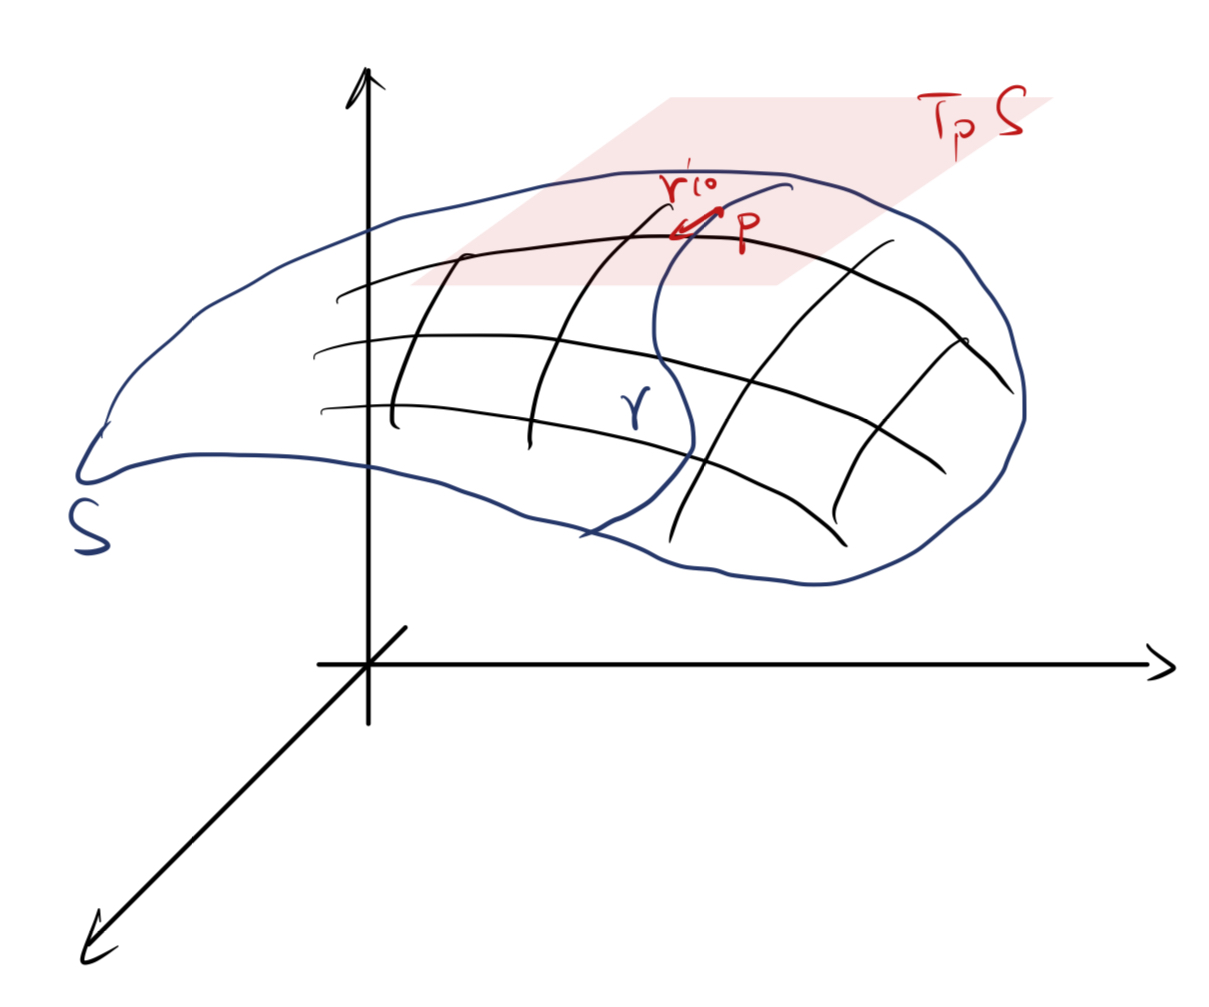
\includegraphics[width=7cm]{attachment/IMG_4115.jpeg}
	\caption{切空间示意图}
\end{figure}

这一定义虽然足够简洁, 却不够自然. 我们会有如下想法: 
\begin{itemize}
	\item 切空间, 几何上来看应当是光滑子流形在某点附近最佳的子向量空间逼近. 这个定义与刚才的定义是否等价? 
	\item 若从函数的角度考虑, 函数在一点的微分是其在该点处最佳的线性映射逼近. 微分与切空间有怎样的关系? 
\end{itemize}

\begin{proposition}{切空间的等价定义}
	
\end{proposition}

\newpage
\section{中值定理与Taylor公式}

\subsection{微分中值定理}

\subsection{Taylor公式}

\subsection{多元函数的极值}

\newpage
\section{隐函数定理}

\subsection{反函数定理}

\subsection{隐函数定理}


\newpage
\section{隐函数定理的应用}

\subsection{流形版本的隐函数定理}

\subsection{Lagrange乘子法}